%=========================================================
% Peripheral : SPI
%=========================================================
\section{Peripheral : SPI}

\begin{description}

    \item[Overview]\mbox{}\\
        This module is a simple master SPI interface based on the OpenCores SPI Interface (https://opencores.org/projects/simple\_spi) by Richard Herveille. Please refer to the IP’s document for more details. The SPI can generate interrupt requests upon completion of transfer blocks specified by the ICNT bits in the SPI\_SPER register. Please control the SPI Chip Select Pin level by directly manipulating the SPI\_SPCS register as if it were a GPIO output port.

    \item[Input / Output Signals]\mbox{}\\
        Input / Output signals of SPI are shown in Table \ref{tb:IOSIGNALS_SPI}. The SPI\_MOSI signal always drives 0 or 1 (not 3-state) because the SPI has only master mode.

%-------------------------------
\begin{table}[H]
    \begin{adjustbox}{scale={0.65}{0.8}}
    \textsf{
    \begin{tabular}{|L{4cm}{2cm}{t}|L{4cm}{2cm}{t}|L{2cm}{1cm}{t}|L{7cm}{6cm}{t}|L{10cm}{6cm}{t}|L{3cm}{2cm}{t}|}
        \hline
        %-------------------------------------
        \rowcolor{LightPurple}
        \textbf{Group} &
        \textbf{Direction} &
        \textbf{Width} &
        \textbf{Name} &
        \textbf{Description} &
        \textbf{Note}
        \nextRow \hline
        %-------------------------------------
        System & input  & ~ & RES & Reset & ~
        \nextRow \hline
        %-------------------------------------
        System & input  & ~ & CLK & System Clock & ~
        \nextRow \hline
        %-------------------------------------
        AHB    & input  & ~                   & S\_HSEL      & AHB Lite Slave Select & ignored
        \nextRow \hline
        %-------------------------------------
        AHB    & input  & \lbrack  1:0\rbrack & S\_HTRANS    & AHB Lite Slave Transfer Type & ~
        \nextRow \hline
        %-------------------------------------
        AHB    & input  & ~                   & S\_HWRITE    & AHB Lite Slave Write & ~
        \nextRow \hline
        %-------------------------------------
        AHB    & input  &                     & S\_HMASTLOCK & AHB Lite Slave Locked Transfer & ignored
        \nextRow \hline
        %-------------------------------------
        AHB    & input  & \lbrack  2:0\rbrack & S\_HSIZE     & AHB Lite Slave Access Size & ~
        \nextRow \hline
        %-------------------------------------
        AHB    & input  & \lbrack  2:0\rbrack & S\_HBURST    & AHB Lite Slave Burst Access & ignored
        \nextRow \hline
        %-------------------------------------
        AHB    & input  & \lbrack  3:0\rbrack & S\_HPROT     & AHB Lite Slave Protection & ignored
        \nextRow \hline
        %-------------------------------------
        AHB    & input  & \lbrack 31:0\rbrack & S\_HADDR     & AHB Lite Slave Address & ~
        \nextRow \hline
        %-------------------------------------
        AHB    & input  & \lbrack 31:0\rbrack & S\_HWDATA    & AHB Lite Slave Write Data & ~
        \nextRow \hline
        %-------------------------------------
        AHB    & input  & ~                   & S\_HREADY    & AHB Lite Slave Ready Input & ~
        \nextRow \hline
        %-------------------------------------
        AHB    & output & ~                   & S\_HREADYOUT & AHB Lite Slave Ready Output & ~
        \nextRow \hline
        %-------------------------------------
        AHB    & output & \lbrack 31:0\rbrack & S\_HRDATA    & AHB Lite Slave Read Data & ~
        \nextRow \hline
        %-------------------------------------
        AHB    & output & ~                   & S\_HRESP     & AHB Lite Slave Response & always output 0
        \nextRow \hline
        %-------------------------------------
        SPI    & output & \lbrack  3:0\rbrack & SPI\_CSN     & SPI Chip Selects & ~
        \nextRow \hline
        %-------------------------------------
        SPI    & output & ~                   & SPI\_SCK     & SPI Clock & ~
        \nextRow \hline
        %-------------------------------------
        SPI    & output & ~                   & SPI\_MOSI    & SPI Master Output / Slave Input & ~
        \nextRow \hline
        %-------------------------------------
        SPI    & input  & ~                   & SPI\_MISO    & SPI Master Input / Slave Output & ~
        \nextRow \hline
        %-------------------------------------
        INT    & output & ~                   & IRQ\_SPI      & Interrupt Request & ~
        \nextRow \hline
        %-------------------------------------
    \end{tabular}
    }
    \end{adjustbox}
    \caption{Input / Output Signals of SPI}
    \label{tb:IOSIGNALS_SPI}
\end{table}
%-------------------------------

    \item[Control Registers]\mbox{}\\
        Controls registers of SPI are shown in Table \ref{tb:REG_I2C_SPCR} to Table \ref{tb:REG_I2C_SPCS}. Please refer the technical document of the OpenCores SPI Interface (https://opencores.org/projects/simple\_spi).
 
\end{description}

%-------------------------------
\begin{table}[H]
    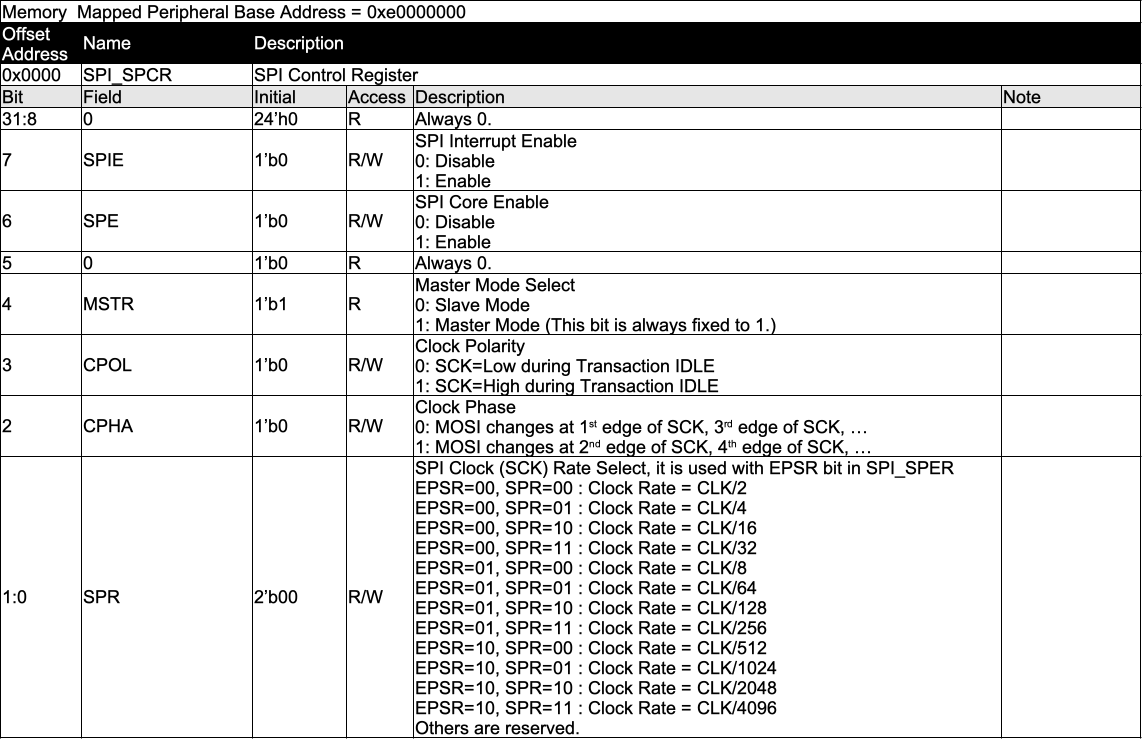
\includegraphics[width=1.0\columnwidth]{./Table/REG_SPI_SPCR.png}
    \caption{I2C\_SPCR}
    \label{tb:REG_I2C_SPCR}
\end{table}
%-------------------------------
%-------------------------------
\begin{table}[H]
    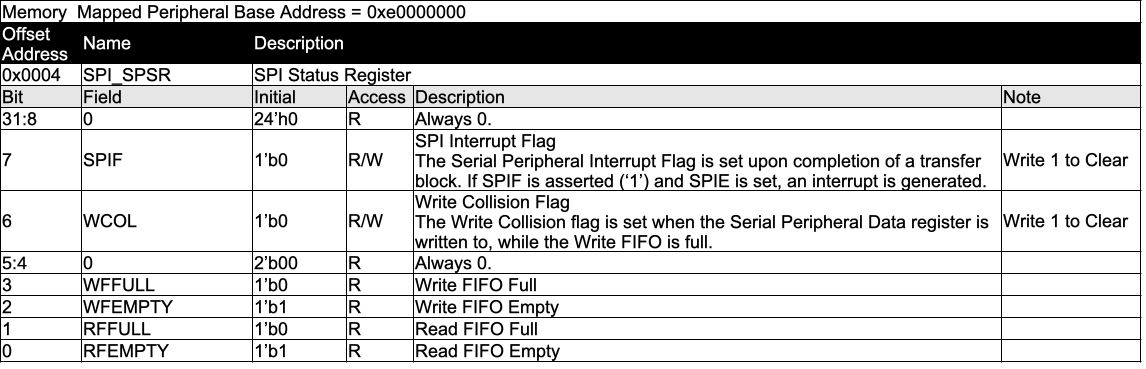
\includegraphics[width=1.0\columnwidth]{./Table/REG_SPI_SPSR.png}
    \caption{I2C\_SPSR}
    \label{tb:REG_I2C_SPSR}
\end{table}
%-------------------------------
%-------------------------------
\begin{table}[H]
    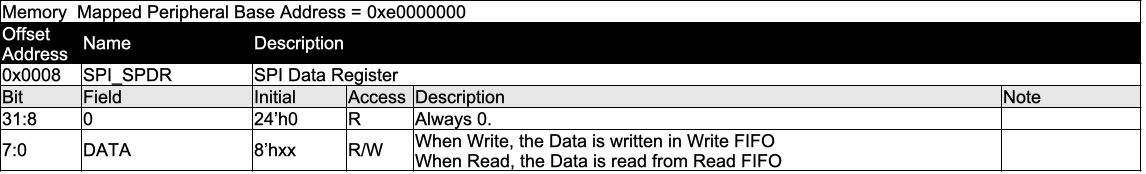
\includegraphics[width=1.0\columnwidth]{./Table/REG_SPI_SPDR.png}
    \caption{I2C\_SPDR}
    \label{tb:REG_I2C_SPDR}
\end{table}
%-------------------------------
%-------------------------------
\begin{table}[H]
    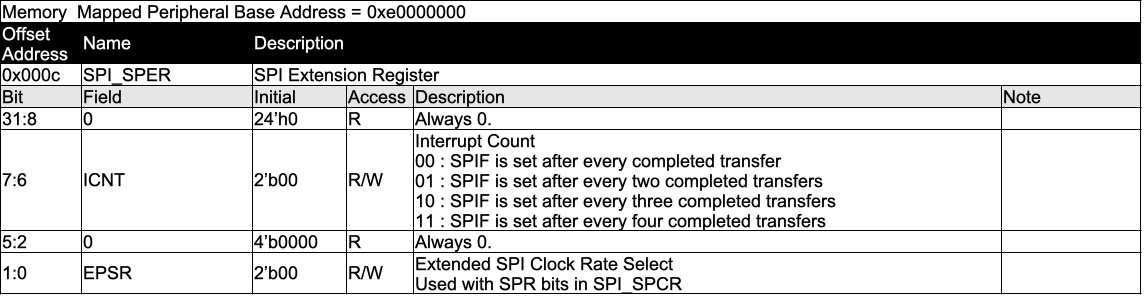
\includegraphics[width=1.0\columnwidth]{./Table/REG_SPI_SPER.png}
    \caption{I2C\_SPER}
    \label{tb:REG_I2C_SPER}
\end{table}
%-------------------------------
%-------------------------------
\begin{table}[H]
    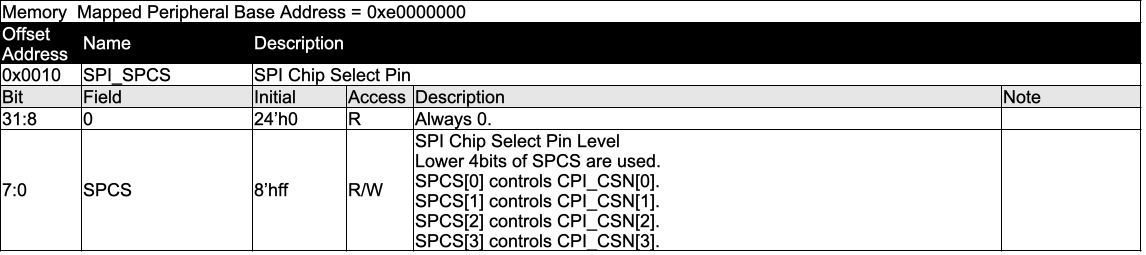
\includegraphics[width=1.0\columnwidth]{./Table/REG_SPI_SPCS.png}
    \caption{I2C\_SPCS}
    \label{tb:REG_I2C_SPCS}
\end{table}
%-------------------------------
